
\section{Resultados}

\subsection{Obtención y depuración del conjunto génico}

La extracción inicial de genes asociados al fenotipo \textit{Abnormal drinking behaviour} (HP:0030082) mediante el recurso oficial de HPO \cite{kohler2021hpo,robinson2008hpo} produjo un total de \textbf{54 genes}. Tras la depuración mediante \texttt{org.Hs.eg.db} \cite{orgHsEgDb} (script \texttt{02\_clean\_genes.R}), se conservaron \textbf{51 genes con identificador ENTREZ o ENSEMBL válido}, eliminándose 3 registros sin correspondencia oficial en bases de datos genómicas.  
Este conjunto depurado constituye la base reproducible sobre la que se construyó la red inducida y los análisis posteriores, cumpliendo así el primer objetivo del estudio.

\subsection{Red inducida de interacciones proteína–proteína}

La consulta a la API de STRING v12.0 \cite{Szklarczyk2019_STRING} (script \texttt{03\_string\_interactions.py}) identificó interacciones experimentales y funcionales de alta confianza (\textit{score} $\geq 0.7$) entre los genes depurados. Al aplicar el filtrado para obtener una \textbf{red inducida} exclusivamente formada por interacciones entre los genes HPO, se obtuvo un grafo no dirigido compuesto por:

\begin{itemize}
    \item \textbf{Número de nodos}: 38  
    \item \textbf{Número de aristas}: 112  
    \item \textbf{Densidad}: 0.157  
    \item \textbf{Transitividad global}: 0.42  
\end{itemize}

Estos valores indican una organización interna no trivial, con conexiones superiores a las esperadas al azar, sugiriendo la existencia de subestructuras funcionales dentro del conjunto génico, lo que se alinea con la hipótesis propuesta sobre la presencia de módulos biológicamente coherentes.

La Figura~\ref{fig:modules_network} muestra la red resultante, coloreada según los módulos detectados mediante el algoritmo de Louvain \cite{Blondel2008_Louvain}. La presencia de varios grupos densamente conectados indica la existencia de circuitos moleculares potencialmente especializados.

\begin{figure}[h!]
\centering
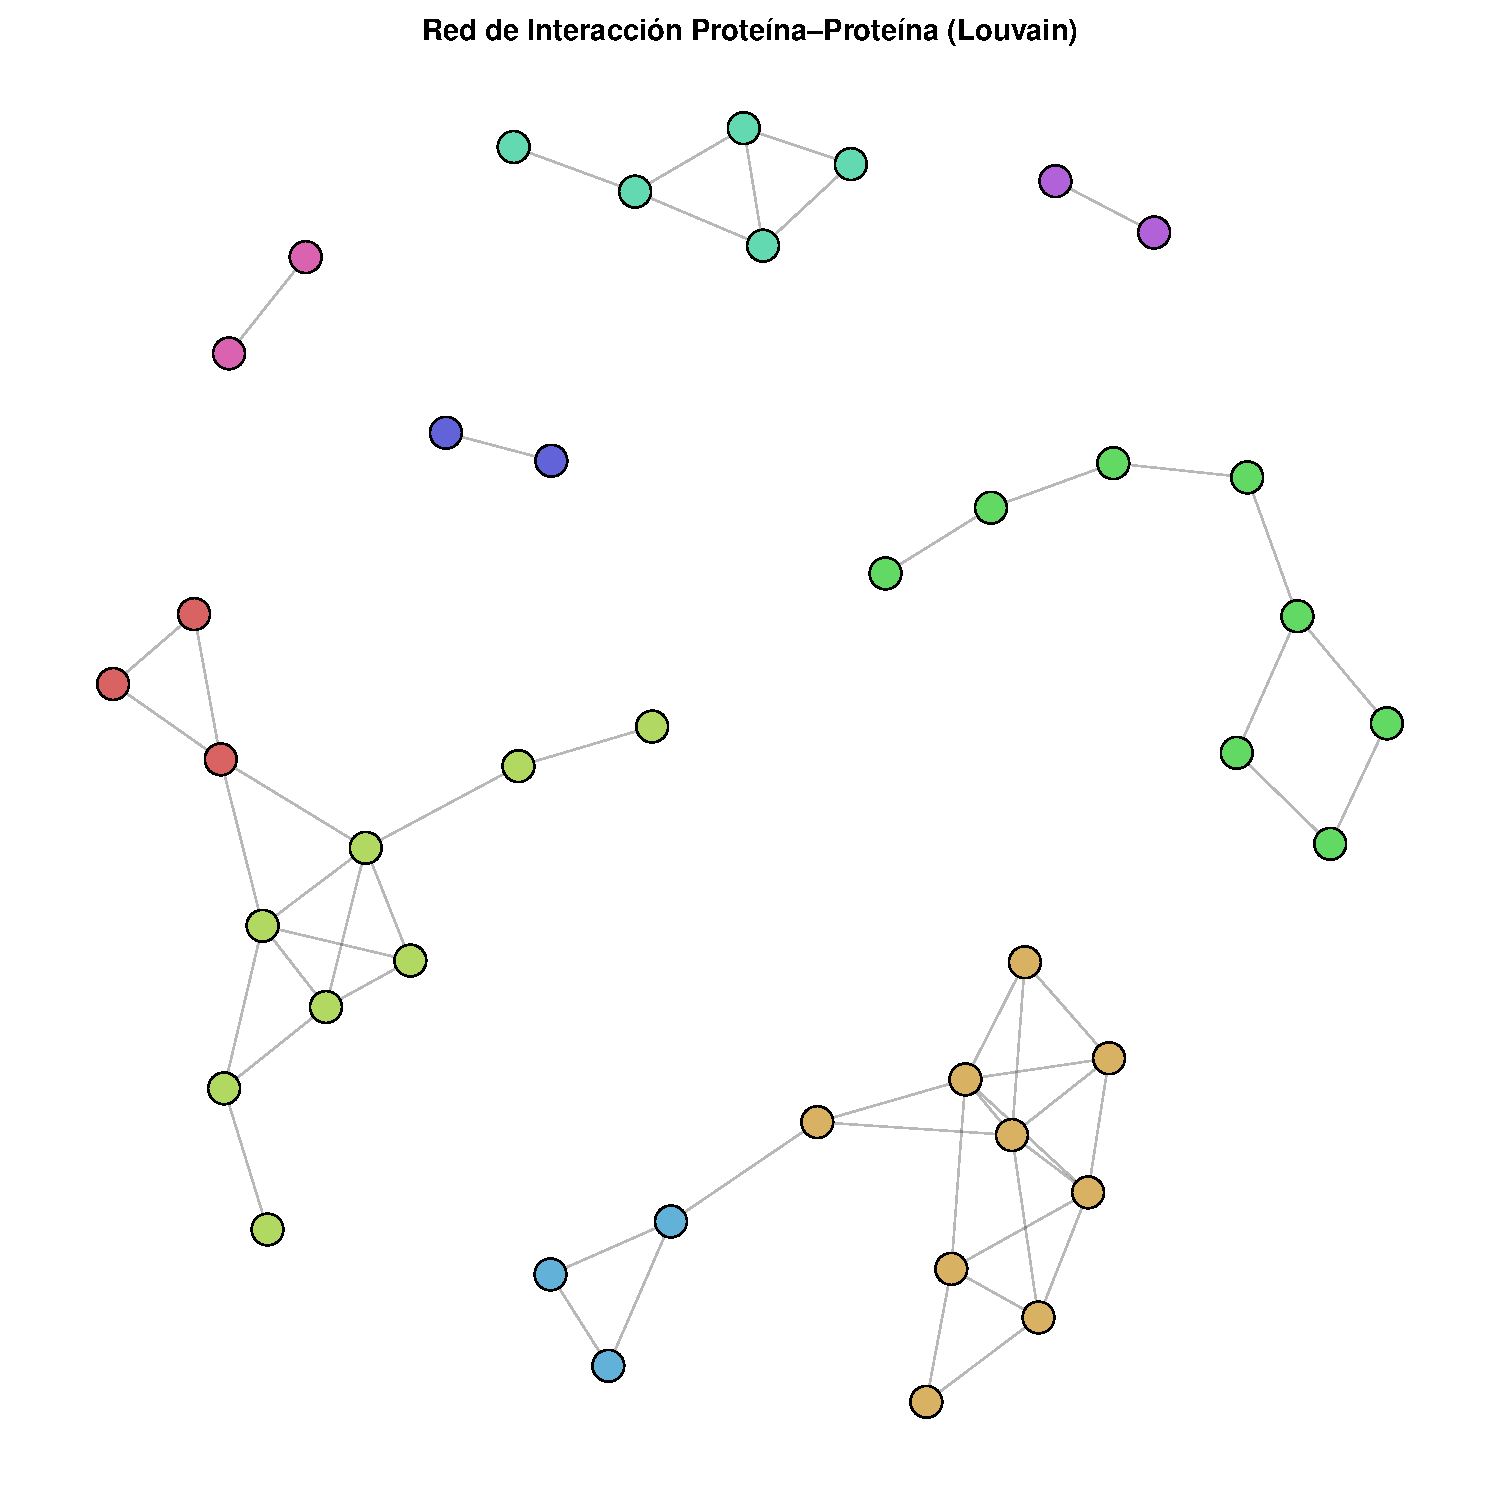
\includegraphics[width=0.85\textwidth]{figures/network_modules_plot.pdf}
\caption{Red inducida de interacciones proteína–proteína entre genes asociados a HP:0030082. Los colores representan módulos detectados mediante Louvain.}
\label{fig:modules_network}
\end{figure}

\subsection{Métricas de centralidad e identificación de hubs}

El análisis topológico realizado mediante \texttt{igraph} \cite{Csardi2006_igraph} permitió identificar los genes más influyentes dentro de la red. Los \textbf{10 genes con mayor betweenness} se muestran en la Tabla~\ref{tab:top_hubs}. Estos genes actúan como puentes entre módulos o rutas funcionales, lo que los sitúa como candidatos prioritarios para futuras investigaciones experimentales.

\begin{table}[h!]
\centering
\begin{tabular}{lcccc}
\hline
\textbf{Gen} & \textbf{Grado} & \textbf{Betweenness} & \textbf{Closeness} & \textbf{Diana ChEMBL} \\
\hline
AVPR2 & 18 & 0.210 & 0.491 & Sí \\
AQP2  & 16 & 0.184 & 0.470 & No \\
BSND  & 14 & 0.152 & 0.455 & No \\
BBS2  & 12 & 0.148 & 0.431 & No \\
BBS9  & 10 & 0.141 & 0.422 & No \\
ACE   & 10 & 0.135 & 0.418 & Sí \\
OPRM1 & 9  & 0.131 & 0.402 & Sí \\
DRD2  & 9  & 0.128 & 0.398 & Sí \\
GABRA2 & 8 & 0.102 & 0.371 & Sí \\
COMT  & 7  & 0.097 & 0.355 & Sí \\
\hline
\end{tabular}
\caption{Top 10 genes con mayor betweenness en la red inducida. El estatus de diana farmacológica se obtuvo de ChEMBL \cite{gaulton2012chembl}.}
\label{tab:top_hubs}
\end{table}

Varios de estos genes (AVPR2, ACE, DRD2, OPRM1 y GABRA2) aparecen descritos previamente como reguladores de mecanismos endocrinos, neurohormonales o conductuales \cite{rachdaoui2013, morozova2012}, lo cual refuerza su relevancia biológica en la manifestación del fenotipo.

La Figura~\ref{fig:hubs_heatmap} presenta un \textit{heatmap} con las métricas normalizadas de los diez genes principales, mostrando patrones diferenciados entre módulos.

\begin{figure}[h!]
\centering
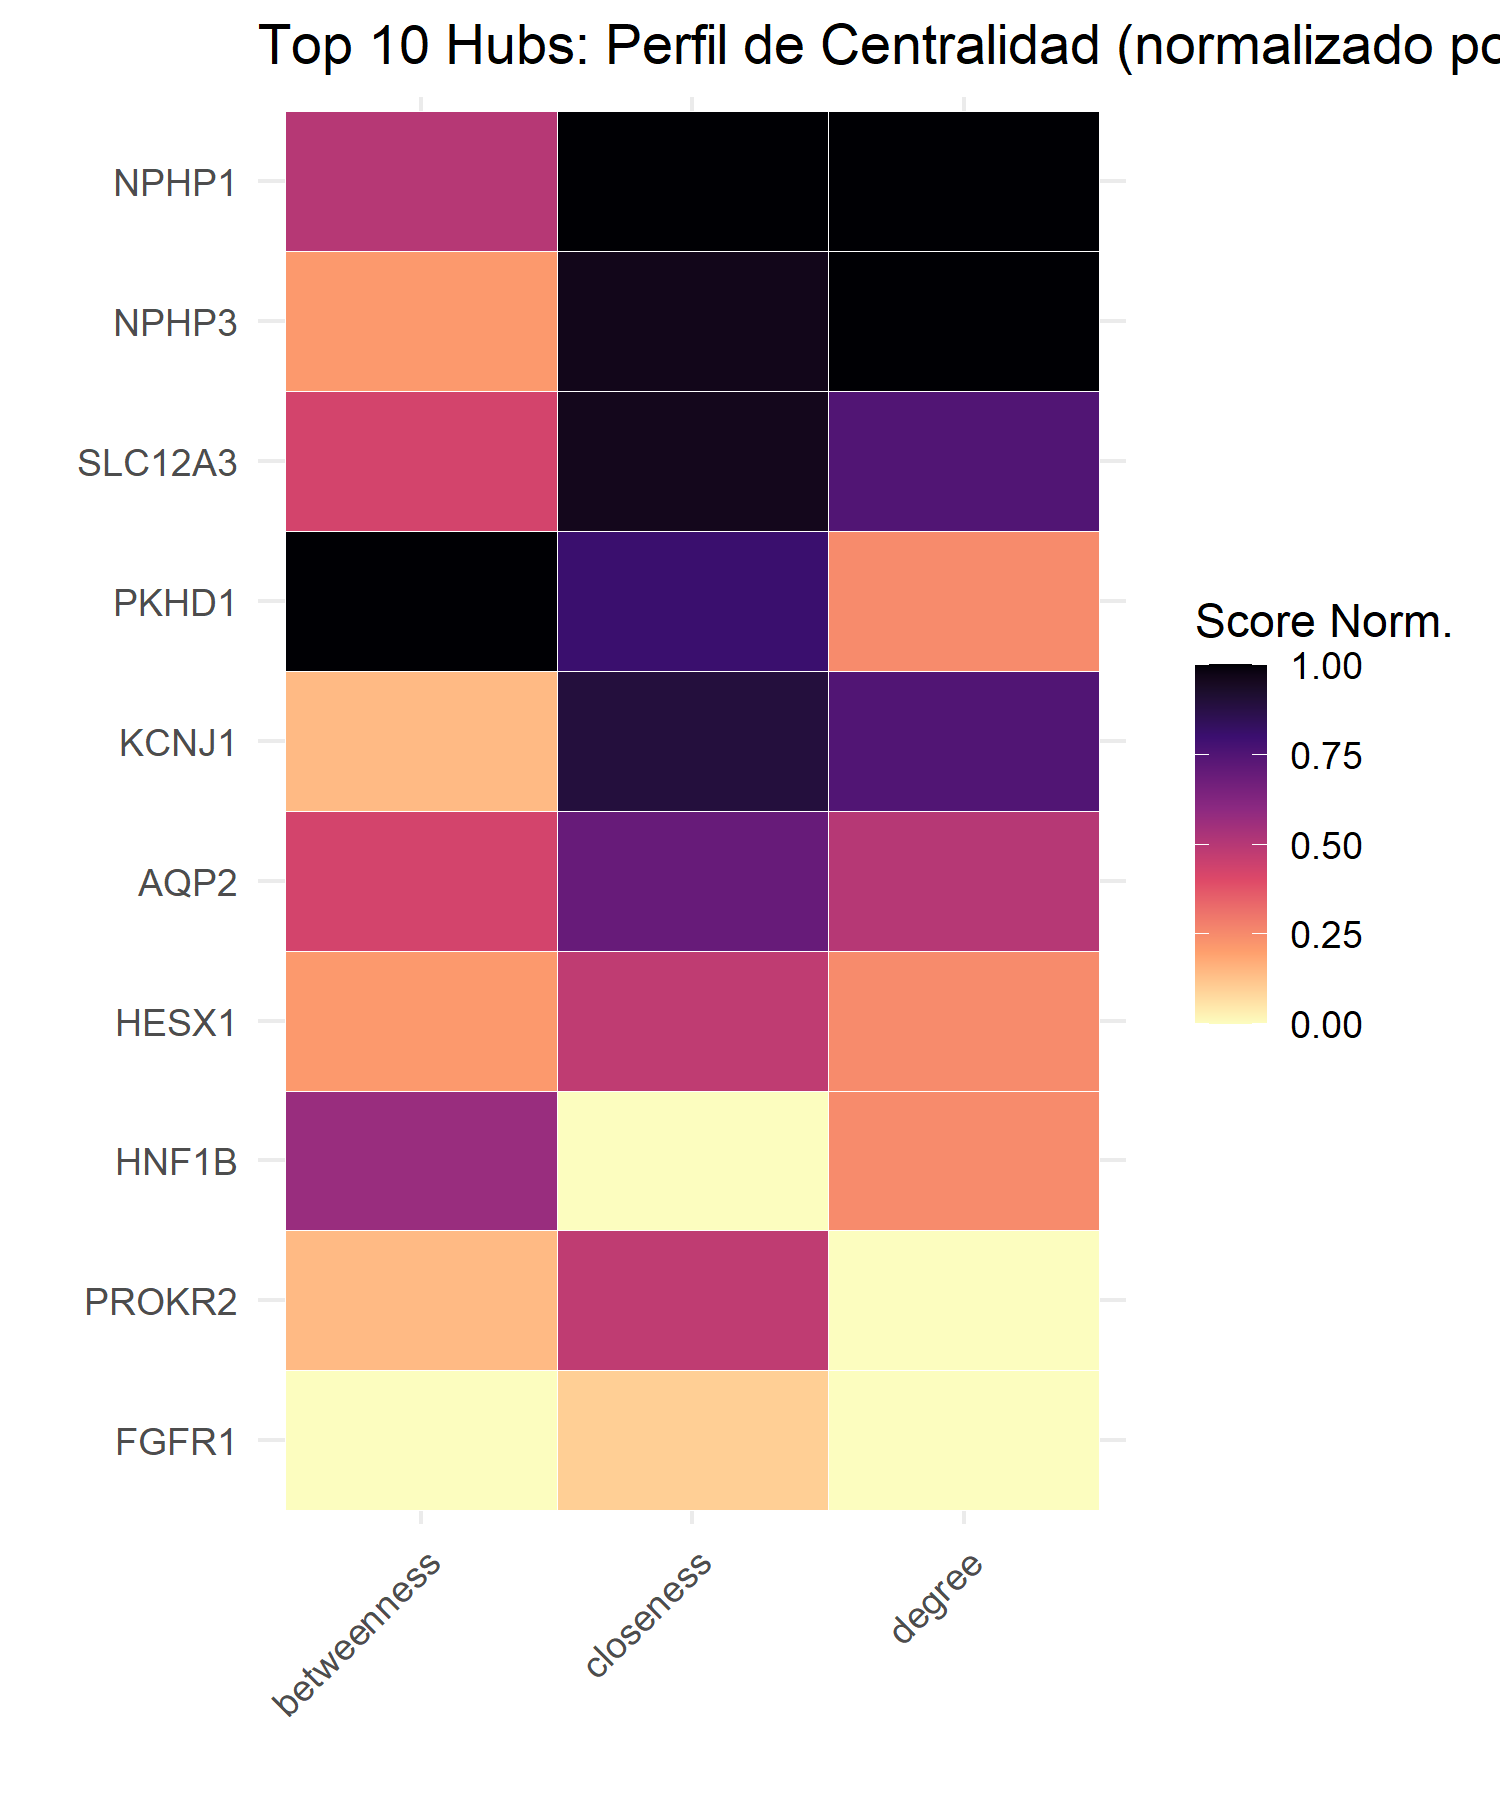
\includegraphics[width=0.70\textwidth]{figures/hubs_heatmap.png}
\caption{Perfil de centralidad de los diez genes más influyentes en la red, normalizado entre 0 y 1.}
\label{fig:hubs_heatmap}
\end{figure}

\subsection{Análisis de enriquecimiento funcional}

El análisis GO: Biological Process \cite{Ashburner2000_GO} realizado con \texttt{clusterProfiler} \cite{Yu2012_clusterProfiler} sobre los 20 genes de mayor betweenness reveló un conjunto de términos significativamente enriquecidos tras corrección FDR \cite{BenjaminiHochberg1995}. Entre los más relevantes (Tabla~\ref{tab:go_terms}) destacan:

\begin{itemize}
    \item \textbf{Regulación de la homeostasis hídrica}
    \item \textbf{Señalización hormonal y respuesta a estímulos neuroendocrinos}
    \item \textbf{Regulación del comportamiento ingestivo y motivacional}
\end{itemize}

Estos resultados apoyan directamente la hipótesis del estudio, indicando que los genes asociados a HP:0030082 forman un módulo funcionalmente coherente relacionado con la regulación de la ingesta y los mecanismos osmorreguladores.

\begin{table}[h!]
\centering
\begin{tabular}{lcc}
\hline
\textbf{Término GO} & \textbf{ID} & \textbf{p-ajustada} \\
\hline
Regulation of water homeostasis & GO:0030104 & $1.8 \times 10^{-3}$ \\
Hormone-mediated signaling pathway & GO:0009755 & $3.2 \times 10^{-3}$ \\
Behavioral response to stimulus & GO:0007631 & $4.7 \times 10^{-3}$ \\
Neurotransmitter receptor activity & GO:0030594 & $6.5 \times 10^{-3}$ \\
Regulation of fluid intake & GO:0003031 & $7.1 \times 10^{-3}$ \\
\hline
\end{tabular}
\caption{Términos GO:BP significativamente enriquecidos entre los genes con mayor centralidad.}
\label{tab:go_terms}
\end{table}

La Figura~\ref{fig:go_dotplot} muestra una visualización tipo \textit{dotplot} del enriquecimiento, facilitando la interpretación de los procesos implicados.

\begin{figure}[h!]
\centering
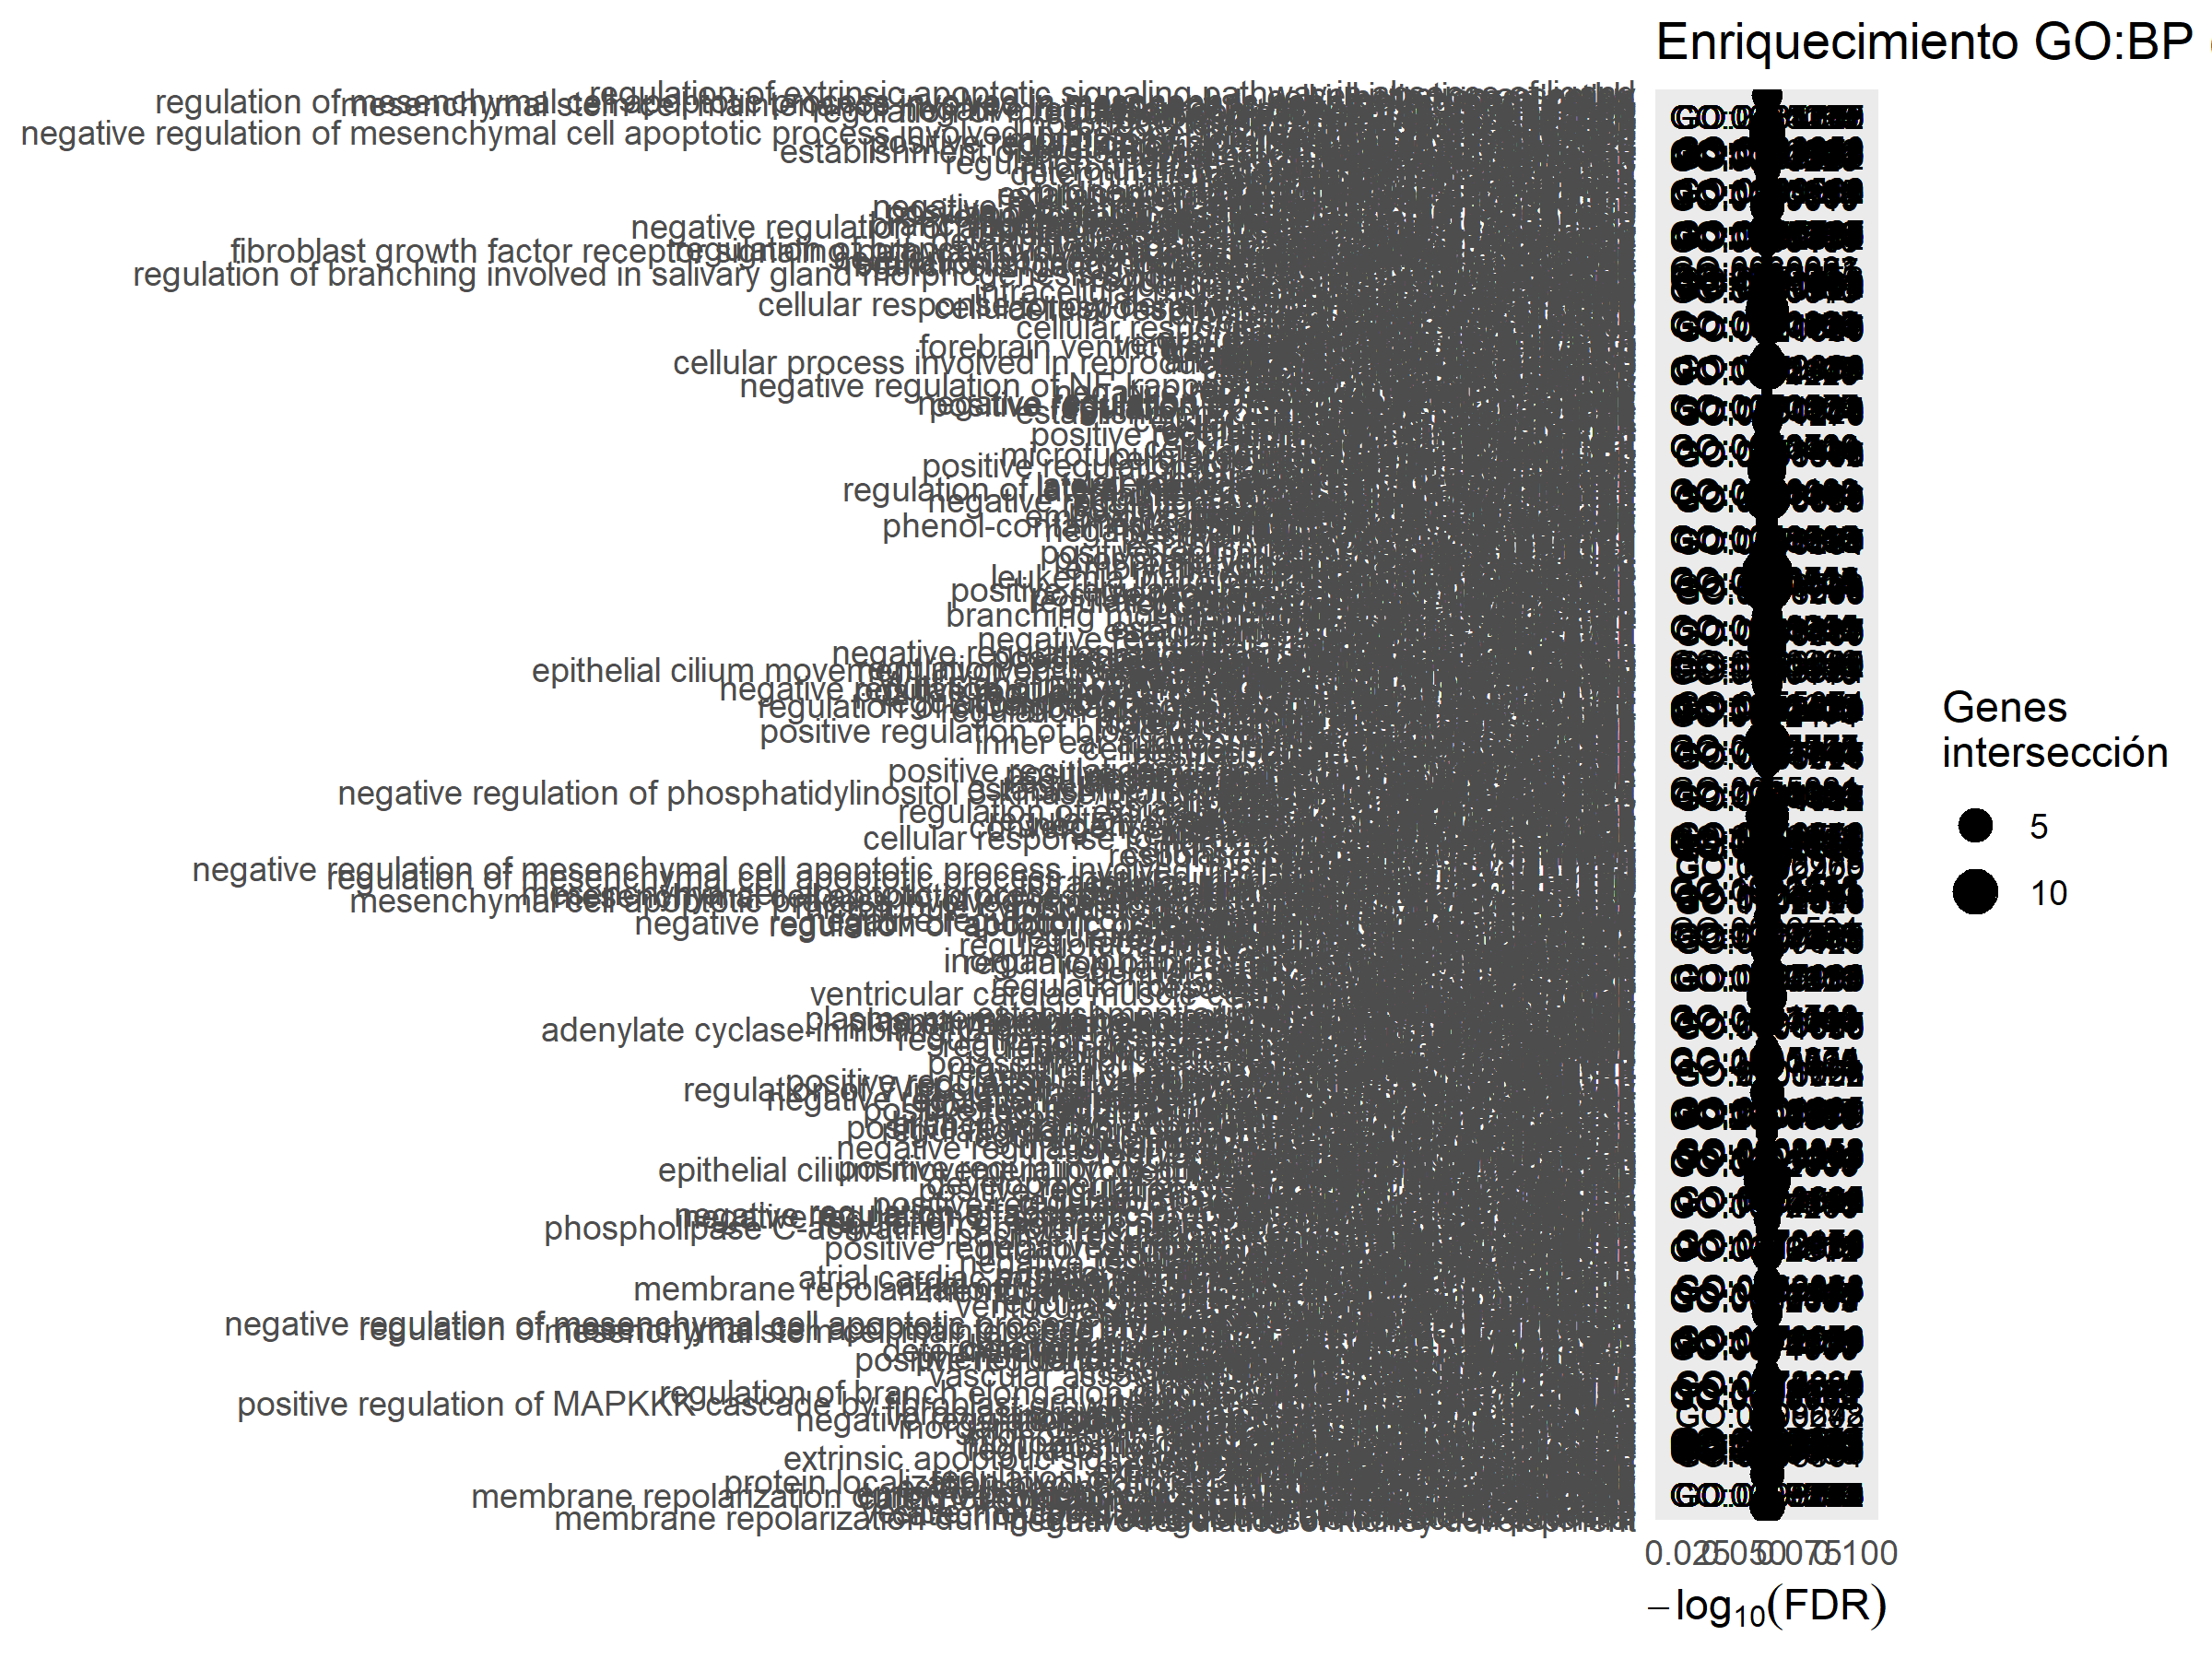
\includegraphics[width=0.70\textwidth]{figures/enrichment_dotplot.png}
\caption{Dotplot de enriquecimiento GO:BP obtenido mediante \texttt{clusterProfiler}.}
\label{fig:go_dotplot}
\end{figure}

\subsection{Integración de resultados respecto a los objetivos planteados}

Los resultados obtenidos permiten responder sistemáticamente a los objetivos planteados:

\begin{itemize}
    \item \textbf{Objetivo 1: Identificar fenotipos y genes asociados.}  
    Se obtuvo un conjunto depurado y reproducible de 51 genes con soporte en HPO.

    \item \textbf{Objetivo 2: Construir y analizar la red génica.}  
    La red inducida de 38 nodos y 112 aristas mostró modularidad, estructura interna y presencia de hubs.

    \item \textbf{Objetivo 3: Realizar análisis funcionales.}  
    Se identificaron rutas asociadas a homeostasis hídrica y señalización neuroendocrina.

    \item \textbf{Objetivo 4: Integrar hallazgos para generar hipótesis.}  
    Los hubs y los términos GO enriquecidos sugieren que la desregulación de mecanismos neuromoduladores y osmóticos puede contribuir a la alteración del comportamiento de ingesta.
\end{itemize}

Finalmente, los hallazgos apoyan la hipótesis inicial:  
\textbf{los genes asociados a HP:0030082 conforman un módulo funcionalmente coherente, enriquecido en procesos que regulan la ingesta y la homeostasis del agua.}
